% !TEX root = ../Tesis.tex
\chapter{Tablas de validación de datos 
de las estaciones de monitoreo de calidad 
del aire}
\label{anexo:tablas_validacion}

En este apéndice se presentan las tablas de criterios, rangos de operación y
límites utilizados para la limpieza y verificación de los datos de calidad
del aire y variables meteorológicas empleados en esta tesis.

\begin{table}[H]
\centering
\footnotesize
\caption{Criterios de asignación de banderas para la limpieza de datos.}
\label{tab:banderas_limpieza}
\begin{tabular}{@{}lL{.78\textwidth}@{}}
\toprule
\textbf{Bandera} & \textbf{Criterio} \\
\midrule
VA & Dato válido: dato que se considera correcto o verdadero pero que
está sujeto a revisión en la etapa de verificación de datos. \\
IC & Dato inválido por calibración: datos que provengan de las
actividades de calibración de los equipos de medición. Asimismo, se
incluirán aquellos datos generados como resultado de la ejecución del
programa de pruebas de cero/span. \\
IR & Dato inválido por rango de operación: valores fuera de los límites
superior e inferior fijados en el equipo de medición
(Tablas~\ref{tab:rangos_operacion} y~\ref{tab:limites_inferiores}). \\
VZ & Dato válido igualado al límite de detección o a cero: datos con
valores negativos que, excepto en el caso de las mediciones de
temperatura, deberán ser igualados a cero o al límite de detección
correspondiente para poderlos incluir en la base de datos revisada. \\
IF & Dato inválido por falla del equipo: datos de los que exista
evidencia en bitácora o en listas de verificación cuyos parámetros de
operación (temperaturas, flujos, presiones, voltajes) se encuentran
fuera de los valores normales de operación. \\
ND & Dato no disponible: se aplica a cualquier dato ausente, ya sea por
fallas en la transmisión-recepción o por cortes de energía. \\
\bottomrule
\end{tabular}
\end{table}

\begin{table}[H]
\centering
\footnotesize
\caption{Rangos de operación por contaminante.}
\label{tab:rangos_operacion}
\begin{tabular}{@{}ll@{}}
\toprule
\textbf{Contaminante} & \textbf{Rango de operación} \\
\midrule
O\textsubscript{3} & 0--500 ppb \\
SO\textsubscript{2} & 0--500 ppb \\
NO\textsubscript{2} & 0--500 ppb \\
NO & 0--500 ppb \\
NO\textsubscript{x} & 0--500 ppb \\
CO & 0--50 ppm \\
Hidrocarburos totales & 0--10 / 0--20 ppmc \\
Metanos & 0--10 / 0--20 ppmc \\
No metanos & 0--10 / 0--20 ppmc \\
Partículas PM\textsubscript{10} & 0--500 / 0--1000 \si{\micro\gram\per\cubic\meter} \\
Partículas PM\textsubscript{2.5} & 0--500 / 0--1000 \si{\micro\gram\per\cubic\meter} \\
Humedad relativa & 0--100\% \\
Presión barométrica & 500--760 mmHg \\
Precipitación pluvial & 0--10 mm \\
Radiación solar & 0--2000 \si{\watt\per\square\meter} \\
Radiación UV-A & 0--300 mW/m\textsuperscript{2} \\
                & 0--2000 mW/m\textsuperscript{2} \\
Radiación UV-B & 0--5 MED/hr \\
                & 0--600 mW/m\textsuperscript{2} \\
Velocidad del viento & 0--50 m/s \\
Dirección del viento & 0--360$^{\circ}$ \\
Temperatura ambiental & $-50$ a $500\,^{\circ}\mathrm{C}$ \\
\bottomrule
\end{tabular}
\end{table}

\begin{table}[H]
\centering
\footnotesize
\caption{Límites inferiores por contaminante.}
\label{tab:limites_inferiores}
\begin{tabular}{@{}ll@{}}
\toprule
\textbf{Contaminante} & \textbf{Mínimo inferior} \\
\midrule
O\textsubscript{3} & $-3$ ppb \\
SO\textsubscript{2} & $-3$ ppb \\
NO\textsubscript{2} & $-3$ ppb \\
NO & $-3$ ppb \\
NO\textsubscript{x} & $-6$ ppb \\
CO & $-0.4$ ppm \\
\bottomrule
\end{tabular}
\end{table}

{\footnotesize
\begin{longtable}{@{}l L{.17\textwidth} L{.62\textwidth}@{}}
\caption{Criterios de asignación de banderas para la verificación de
datos.}\label{tab:banderas_verificacion}\\
\toprule
\textbf{Bandera} & \textbf{Significado} & \textbf{Criterio} \\
\midrule
\endfirsthead
\multicolumn{3}{@{}l}{\textit{Tabla~\thetable\ (continuación)}} \\
\toprule
\textbf{Bandera} & \textbf{Significado} & \textbf{Criterio} \\
\midrule
\endhead
\midrule
\multicolumn{3}{r}{\textit{Continúa en la página siguiente}} \\
\endfoot
\bottomrule
\endlastfoot
DS & Dato sospechoso &
Cuando existen valores constantes por más de tres horas consecutivas
de CO, NO\textsubscript{x}, NO\textsubscript{2}, NO,
O\textsubscript{3}, SO\textsubscript{2}, PM\textsubscript{10} o
PM\textsubscript{2.5}. \\
\midrule
IO & Inválido por operador &
Cuando la suma de NO y NO\textsubscript{2} dividida entre
NO\textsubscript{x} se encuentra fuera del intervalo $(0.85,\,1.15)$. \\
   & &
Cuando la relación de PM\textsubscript{2.5} entre PM\textsubscript{10}
es mayor a $1.15$. \\
   & &
Para datos de radiación (total, UVA, UVB, UVC) cuando esta es diferente
a cero durante la noche. \\
   & &
Para datos de velocidad de viento cuando esta no varía en más de
$0.1$\,m/s en tres horas consecutivas o en más de $0.5$\,m/s en doce
horas consecutivas. \\
   & &
Cuando los datos de dirección de viento no varían en más de
$1^{\circ}$ por más de tres horas consecutivas o en más de
$10^{\circ}$ durante dieciocho horas consecutivas. \\
   & &
Cuando los datos de temperatura cambian en más de
$5\,^{\circ}\mathrm{C}$ respecto a la hora previa o no varían en más de
$0.5\,^{\circ}\mathrm{C}$ en doce horas consecutivas. \\
   & &
Para datos de presión barométrica cuando esta tiene cambios de más de
$0.75$\,mmHg en tres horas consecutivas. \\
\midrule
VC & Dato válido calculado &
Se usa en aquellos datos que son obtenidos por medio de interpolación o
por el uso de series de tiempo. También es aplicable a aquellos que son
corregidos de acuerdo con los resultados de las verificaciones de cero
y \textit{span}. \\
\midrule
VE & Dato válido con evento extraordinario &
Se aplica para datos cuya frecuencia y duración fueron registrados en
la bitácora general de operación. También cuando existe evidencia
documental de eventos que afectaron la medición, tales como incendios,
tolvaneras o actividades de construcción. \\
\midrule
DV & Dato para verificar &
Bandera temporal que incluye datos que deberán ser confirmados en alguna
de las categorías anteriores. También se puede asignar esta bandera a
datos que se presentan fuera de los límites establecidos con base en
tendencias históricas de cada uno de los contaminantes medidos o
parámetros meteorológicos. \\
\end{longtable}}

\chapter{Evaluación de contaminantes atmosféricos en Salamanca, Guanajuato
(2023)}
\label{anexo:graf_historico}

\begin{figure}[H]
    \centering
    % Fila 1
    \begin{subfigure}[t]{0.49\textwidth}
        \centering
        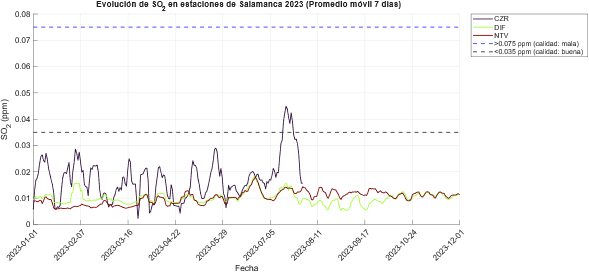
\includegraphics[width=\linewidth]{Anexos/SO2_Salamanca2023.png}
        \caption{SO$_2$}
        \label{fig:anexo_so2_serie}
    \end{subfigure}
    \hfill
    \begin{subfigure}[t]{0.49\textwidth}
        \centering
        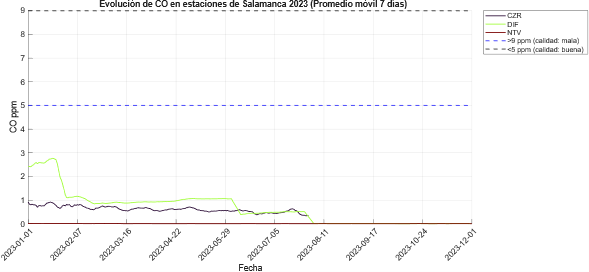
\includegraphics[width=\linewidth]{Anexos/CO_Salamanca2023.png}
        \caption{CO}
        \label{fig:anexo_co_serie}
    \end{subfigure}

    \vspace{0.8em}

    % Fila 2
    \begin{subfigure}[t]{0.49\textwidth}
        \centering
        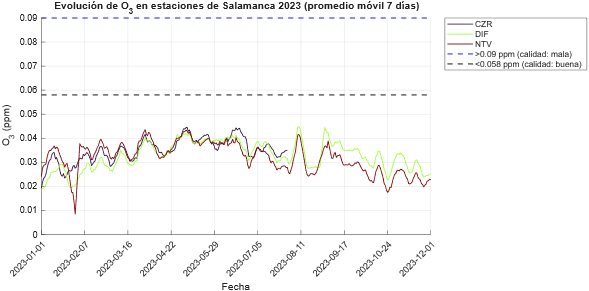
\includegraphics[width=\linewidth]{Anexos/O3_Salamanca2023.png}
        \caption{O$_3$}
        \label{fig:anexo_o3_serie}
    \end{subfigure}
    \hfill
    \begin{subfigure}[t]{0.49\textwidth}
        \centering
        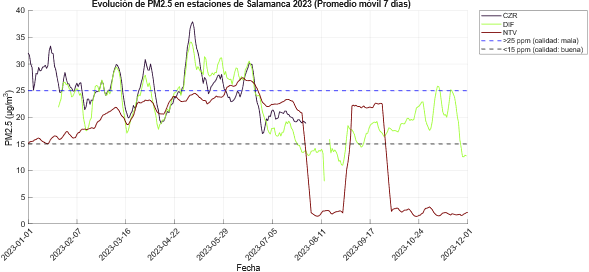
\includegraphics[width=\linewidth]{Anexos/PM2_5_Salamanca2023.png}
        \caption{PM$_{2.5}$}
        \label{fig:anexo_pm25_serie}
    \end{subfigure}

    \vspace{0.8em}

    % Fila 3 (imagen centrada)
    \begin{subfigure}[t]{0.49\textwidth}
        \centering
        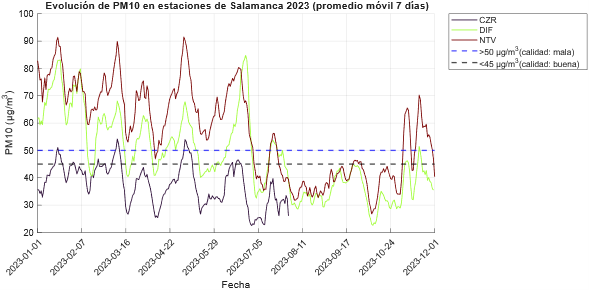
\includegraphics[width=\linewidth]{Anexos/PM10_Salamanca2023.png}
        \caption{PM$_{10}$}
        \label{fig:anexo_pm10_serie}
    \end{subfigure}

    \caption{Evolución de SO$_2$, CO, O$_3$, PM$_{2.5}$ y PM$_{10}$ en las estaciones CZR, DIF y NTV de Salamanca durante 2023 (promedio móvil de 7 días). Las líneas punteadas indican los umbrales de calidad del aire buena y mala.}
    \label{fig:anexo_series}
\end{figure}

\begin{figure}[H]
    \centering
    % Fila 1
    \begin{subfigure}[t]{0.49\textwidth}
        \centering
        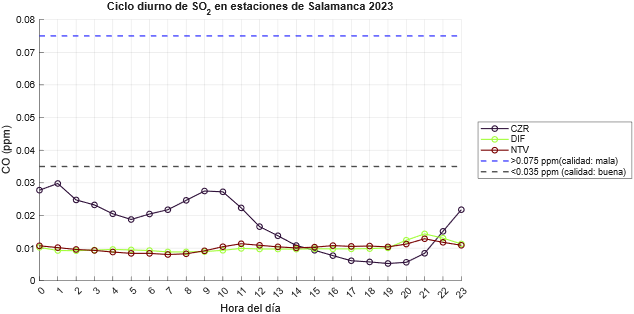
\includegraphics[width=\linewidth]{Anexos/CicloDiruno_SO2_Salamanca2023.png}
        \caption{SO$_2$}
        \label{fig:anexo_so2_ciclo}
    \end{subfigure}
    \hfill
    \begin{subfigure}[t]{0.49\textwidth}
        \centering
        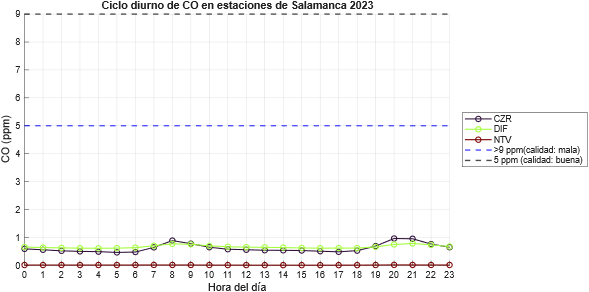
\includegraphics[width=\linewidth]{Anexos/CicloDiruno_CO_Salamanca2023.png}
        \caption{CO}
        \label{fig:anexo_co_ciclo}
    \end{subfigure}

    \vspace{0.8em}

    % Fila 2
    \begin{subfigure}[t]{0.49\textwidth}
        \centering
        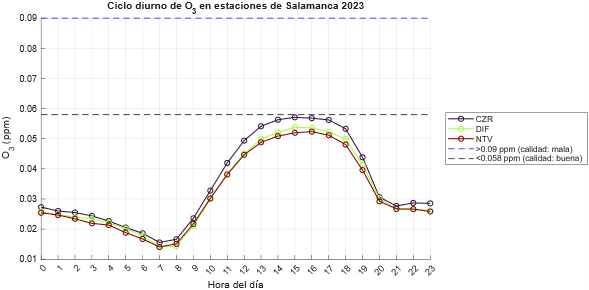
\includegraphics[width=\linewidth]{Anexos/CicloDiurno_O3_Salamanca2023.png}
        \caption{O$_3$}
        \label{fig:anexo_o3_ciclo}
    \end{subfigure}
    \hfill
    \begin{subfigure}[t]{0.49\textwidth}
        \centering
        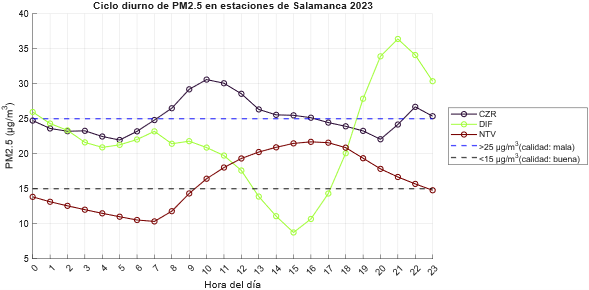
\includegraphics[width=\linewidth]{Anexos/CicloDiurno_PM2_5_Salamanca2023.png}
        \caption{PM$_{2.5}$}
        \label{fig:anexo_pm25_ciclo}
    \end{subfigure}

    \vspace{0.8em}

    % Fila 3 (imagen centrada)
    \begin{subfigure}[t]{0.49\textwidth}
        \centering
        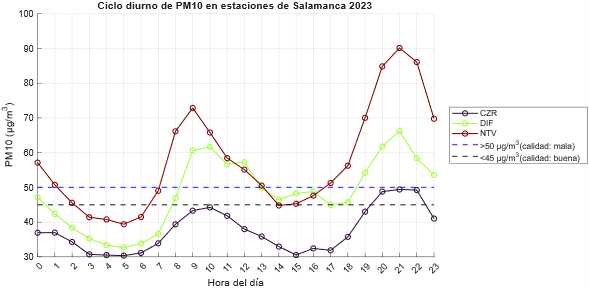
\includegraphics[width=\linewidth]{Anexos/CicloDiurno_PM10_Salamanca2023.png}
        \caption{PM$_{10}$}
        \label{fig:anexo_pm10_ciclo}
    \end{subfigure}

    \caption{Ciclos diurnos de SO$_2$, CO, O$_3$, PM$_{2.5}$ y PM$_{10}$ en las estaciones CZR, DIF y NTV de Salamanca durante 2023.}
    \label{fig:anexo_ciclos}
\end{figure}

\chapter{Tabla de referencia de las industrias de Salamanca
consideradas en el modelo de FLEXPART}
\label{anexo:indus_num}

\begin{longtable}{r l p{7.5cm} r r}
\caption{Establecimientos industriales con su clave, razón social y coordenadas geográficas.}
\label{tab:empresas} \\
\toprule
\textbf{No.} & \textbf{Clave} & \textbf{Nombre de la empresa o razón social} & \textbf{Lat (N)} & \textbf{Lon (W)} \\
\midrule
\endfirsthead

\multicolumn{5}{c}{\tablename\ \thetable\ (continuación)} \\
\toprule
\textbf{No.} & \textbf{Clave} & \textbf{Nombre de la empresa o razón social} & \textbf{Lat (N)} & \textbf{Lon (W)} \\
\midrule
\endhead

\midrule
\multicolumn{5}{r}{\textit{Continúa en la siguiente página}} \\
\endfoot

\bottomrule
\endlastfoot

1  & AEB325999112700 & ACEITES Y ESPECIALIDADES DEL BAJÍO, S.A. de C.V. & 20.56151714 & $-$101.160542 \\
2  & DTM327111112700 & DAL-TILE MÉXICO, S. de R.L. de C.V. & 20.52271842 & $-$101.2104653 \\
3  & FEP324120112700 & FABRICACIÓN DE EMULSIONES Y PAVIMENTOS DE GUERRERO, S.A. de C.V. & 20.54088237 & $-$101.1153477 \\
4  & ACE336320112700 & FUJIKURA AUTOMOTIVE MÉXICO QUERÉTARO, S.A. de C.V. & 20.54591031 & $-$101.1204875 \\
5  & ITI327122112700 & IBÉRICA TILES, S.A.P.I. de C.V. & 20.52255752 & $-$101.2088114 \\
6  & JCS336390112700 & J CLIMA SISTEMAS MÉXICO, S.A. de C.V. & 20.62063182 & $-$101.2346097 \\
7  & PME336390112700 & PENSTONE MEXICANA, S.A. de C.V. & 20.61706994 & $-$101.2324565 \\
8  & PFR311411112000 & PRODUCTOS FRUGO, S.A. de C.V. & 20.59581548 & $-$101.1821423 \\
9  & RSM339999112700 & SATUS AGER MÉXICO, S. de R.L. de C.V. & 20.52116907 & $-$101.2159504 \\
10 & PLO1102700112   & PEMEX LOGÍSTICA -- TERMINAL DE ALMACENAMIENTO Y DESPACHO SALAMANCA & 20.576048 & $-$101.182816 \\
11 & PLO1102700117   & PEMEX LOGÍSTICA & 20.555657 & $-$101.124875 \\
12 & PTI1102700059   & PEMEX TRANSFORMACIÓN INDUSTRIAL, REFINERÍA SALAMANCA (ING. ANTONIO M. AMOR) & 20.58396 & $-$101.178102 \\
13 & TPL1102700153   & TRACTOCOMBUSTIBLES PLAZA, S.A. de C.V. & 20.57196951 & $-$101.180615 \\
14 & CGI1102700159   & CFE GENERACIÓN I, CENTRAL TERMOELÉCTRICA SALAMANCA & 20.567778 & $-$101.17117 \\
15 & CGI1102700202   & CFE GENERACIÓN I, CENTRAL CICLO COMBINADO COGENERACIÓN SALAMANCA & 20.579571 & $-$101.163682 \\
16 & CBLLU1102711    & CARBOQUÍMICA BLOCK, S.A. de C.V. & 20.5397838 & $-$101.1127397 \\
17 & GTK1102700007   & Y-TEC KEYLEX MEXICO, S.A. de C.V. & 20.61592653 & $-$101.2349314 \\
18 & HCA5X1102711    & HENKEL CAPITAL, S.A. de C.V. & 20.55642276 & $-$101.1519663 \\
19 & MMM1102700005   & MAZDA MOTOR MANUFACTURING DE MÉXICO, S.A. de C.V. & 20.60913679 & $-$101.2385826 \\

\end{longtable}

\chapter{Tablas de resultados de la prueba de normalidad}
\label{anexo:normal}

\begin{longtable}{@{}llrrrccc@{}}
\caption{Resultados de las pruebas de normalidad por estación y variable en la campaña de febrero. Se reportan el número de observaciones ($n$), el coeficiente de asimetría, la curtosis y los valores de $p$ de las pruebas de Shapiro-Wilk (S-W), Lilliefors (Lil.) y Anderson-Darling (A-D).}
\label{tab:normalidad_feb}\\
\toprule
Estación & Variable & $n$ & Asimetría & Curtosis & $p$ (S-W) & $p$ (Lil.) & $p$ (A-D) \\
\midrule
\endfirsthead

\multicolumn{8}{c}{\tablename~\thetable{} (continuación)}\\
\toprule
Estación & Variable & $n$ & Asimetría & Curtosis & $p$ (S-W) & $p$ (Lil.) & $p$ (A-D) \\
\midrule
\endhead

\midrule
\multicolumn{8}{r}{\textit{Continúa en la siguiente página}}\\
\endfoot

\bottomrule
\endlastfoot

CR        & O$_3$ (ppb)                      & 297 & 0.21 & 2.21  & $<0.001$ & 0.005       & $<0.001$ \\
          & SO$_2$ (ppb)                     & 308 & 1.80 & 5.62  & $<0.001$ & $\leq0.001$ & $<0.001$ \\
          & CO (ppm)                         & 291 & 1.68 & 6.18  & $<0.001$ & $\leq0.001$ & $<0.001$ \\
          & NO$_2$ (ppb)                     & 308 & 0.54 & 3.05  & $<0.001$ & 0.0014      & $<0.001$ \\
          & PM$_{10}$ ($\mu$g\,m$^{-3}$)     & 303 & 1.15 & 5.18  & $<0.001$ & $\leq0.001$ & $<0.001$ \\
          & PM$_{2.5}$ ($\mu$g\,m$^{-3}$)    & 312 & 0.79 & 3.60  & $<0.001$ & $\leq0.001$ & $<0.001$ \\
          & WS (m\,s$^{-1}$)                 & 312 & 1.18 & 4.46  & $<0.001$ & $\leq0.001$ & $<0.001$ \\
          & Temp ($^{\circ}$C)               & 312 & 0.00 & 2.10  & $<0.001$ & 0.018       & $<0.001$ \\
          & HR (\%)                          & 310 & 0.45 & 2.43  & $<0.001$ & $\leq0.001$ & $<0.001$ \\
\midrule
NATIVITAS & O$_3$ (ppb)                      & 307 & 0.18 & 2.24  & $<0.001$ & 0.120       & 0.002 \\
          & SO$_2$ (ppb)                     & 279 & 2.54 & 12.51 & $<0.001$ & $\leq0.001$ & $<0.001$ \\
          & CO (ppm)                         & 201 & $-0.17$ & 2.85 & $<0.001$ & $\leq0.001$ & $<0.001$ \\
          & NO$_2$ (ppb)                     & 311 & 1.28 & 3.94  & $<0.001$ & $\leq0.001$ & $<0.001$ \\
          & PM$_{10}$ ($\mu$g\,m$^{-3}$)     & 168 & 1.04 & 3.93  & $<0.001$ & $\leq0.001$ & $<0.001$ \\
          & PM$_{2.5}$ ($\mu$g\,m$^{-3}$)    & 265 & $-0.11$ & 2.52 & 0.008   & 0.264       & 0.038 \\
          & WS (m\,s$^{-1}$)                 & 312 & 1.25 & 4.53  & $<0.001$ & $\leq0.001$ & $<0.001$ \\
          & Temp ($^{\circ}$C)               & 312 & $-0.10$ & 2.14 & $<0.001$ & 0.024      & $<0.001$ \\
          & HR (\%)                          & 312 & 0.40 & 2.28  & $<0.001$ & 0.006       & $<0.001$ \\
\midrule
DIF       & O$_3$ (ppb)                      & 281 & 0.28 & 2.09  & $<0.001$ & 0.006       & $<0.001$ \\
          & SO$_2$ (ppb)                     & 253 & 3.37 & 19.62 & $<0.001$ & $\leq0.001$ & $<0.001$ \\
          & CO (ppm)                         & 268 & 1.94 & 9.08  & $<0.001$ & $\leq0.001$ & $<0.001$ \\
          & NO$_2$ (ppb)                     & 281 & 1.20 & 4.13  & $<0.001$ & $\leq0.001$ & $<0.001$ \\
          & PM$_{10}$ ($\mu$g\,m$^{-3}$)     & 275 & 1.28 & 5.41  & $<0.001$ & $\leq0.001$ & $<0.001$ \\
          & PM$_{2.5}$ ($\mu$g\,m$^{-3}$)    & 258 & 0.03 & 2.57  & 0.146    & 0.223       & 0.284 \\
          & WS (m\,s$^{-1}$)                 & 278 & 1.35 & 5.57  & $<0.001$ & $\leq0.001$ & $<0.001$ \\
          & Temp ($^{\circ}$C)               & 283 & $-0.02$ & 2.04 & $<0.001$ & 0.004      & $<0.001$ \\
          & HR (\%)                          & 283 & 0.54 & 2.42  & $<0.001$ & $\leq0.001$ & $<0.001$ \\
\end{longtable}

\begin{longtable}{@{}llrrrccc@{}}
\caption{Resultados de las pruebas de normalidad por estación y variable en la campaña de mayo. Se reportan el número de observaciones ($n$), el coeficiente de asimetría, la curtosis y los valores de $p$ de las pruebas de Shapiro-Wilk (S-W), Lilliefors (Lil.) y Anderson-Darling (A-D).}
\label{tab:normalidad_may}\\
\toprule
Estación & Variable & $n$ & Asimetría & Curtosis & $p$ (S-W) & $p$ (Lil.) & $p$ (A-D) \\
\midrule
\endfirsthead

\multicolumn{8}{c}{\tablename~\thetable{} (continuación)}\\
\toprule
Estación & Variable & $n$ & Asimetría & Curtosis & $p$ (S-W) & $p$ (Lil.) & $p$ (A-D) \\
\midrule
\endhead

\midrule
\multicolumn{8}{r}{\textit{Continúa en la siguiente página}}\\
\endfoot

\bottomrule
\endlastfoot

CR        & O$_3$ (ppb)                      & 120 & 0.44 & 2.53  & 0.010    & 0.132       & 0.018 \\
          & SO$_2$ (ppb)                     & 120 & 2.73 & 12.45 & $<0.001$ & $\leq0.001$ & $<0.001$ \\
          & CO (ppm)                         & 120 & 0.80 & 3.82  & 0.002    & 0.033       & 0.004 \\
          & NO$_2$ (ppb)                     & 106 & 0.60 & 2.01  & $<0.001$ & $\leq0.001$ & $<0.001$ \\
          & PM$_{10}$ ($\mu$g\,m$^{-3}$)     & 119 & 2.66 & 17.58 & $<0.001$ & $\leq0.001$ & $<0.001$ \\
          & PM$_{2.5}$ ($\mu$g\,m$^{-3}$)    & 120 & 0.45 & 3.64  & 0.070    & 0.007       & 0.100 \\
          & WS (m\,s$^{-1}$)                 & 120 & 0.51 & 3.18  & 0.051    & 0.057       & 0.094 \\
          & Temp ($^{\circ}$C)               & 120 & 0.12 & 1.76  & $<0.001$ & 0.015       & $<0.001$ \\
          & HR (\%)                          & 120 & 0.42 & 2.27  & $<0.001$ & 0.088       & 0.002 \\
\midrule
NATIVITAS & O$_3$ (ppb)                      & 120 & 0.36 & 2.32  & 0.015    & 0.002       & 0.009 \\
          & SO$_2$ (ppb)                     & 120 & 3.84 & 19.69 & $<0.001$ & $\leq0.001$ & $<0.001$ \\
          & CO (ppm)                         & 120 & 4.82 & 37.04 & $<0.001$ & $\leq0.001$ & $<0.001$ \\
          & NO$_2$ (ppb)                     & 120 & 1.90 & 8.19  & $<0.001$ & $\leq0.001$ & $<0.001$ \\
          & PM$_{10}$ ($\mu$g\,m$^{-3}$)     & 120 & 1.78 & 8.29  & $<0.001$ & $\leq0.001$ & $<0.001$ \\
          & PM$_{2.5}$ ($\mu$g\,m$^{-3}$)    & 120 & 0.71 & 3.38  & 0.005    & 0.078       & 0.010 \\
          & WS (m\,s$^{-1}$)                 & 120 & 0.64 & 2.08  & $<0.001$ & $\leq0.001$ & $<0.001$ \\
          & Temp ($^{\circ}$C)               & 120 & 0.48 & 2.42  & $<0.001$ & 0.091       & 0.003 \\
\midrule
DIF       & O$_3$ (ppb)                      & 120 & 0.56 & 2.40  & $<0.001$ & $\leq0.001$ & $<0.001$ \\
          & SO$_2$ (ppb)                     & 120 & 3.43 & 14.39 & $<0.001$ & $\leq0.001$ & $<0.001$ \\
          & CO (ppm)                         & 115 & $-0.47$ & 2.86 & $<0.001$ & $\leq0.001$ & $<0.001$ \\
          & NO$_2$ (ppb)                     & 120 & 1.61 & 8.19  & $<0.001$ & $\leq0.001$ & $<0.001$ \\
          & PM$_{10}$ ($\mu$g\,m$^{-3}$)     & 120 & 0.49 & 3.29  & 0.067    & 0.205       & 0.089 \\
          & PM$_{2.5}$ ($\mu$g\,m$^{-3}$)    & 115 & 0.96 & 4.82  & $<0.001$ & 0.003       & 0.005 \\
          & WS (m\,s$^{-1}$)                 & 118 & 0.73 & 3.42  & 0.004    & 0.012       & 0.011 \\
          & Temp ($^{\circ}$C)               & 120 & 0.07 & 1.78  & $<0.001$ & 0.013       & $<0.001$ \\
          & UV                               & 120 & 0.79 & 2.01  & $<0.001$ & $\leq0.001$ & $<0.001$ \\
          & HR (\%)                          & 120 & 0.42 & 2.34  & $<0.001$ & 0.067       & 0.003 \\
\end{longtable}

\chapter{Tablas de resultados de prueba de Friedman}
\label{anexo:fried}

\begin{table}[htbp]
\centering
\caption{Mediana de las variables en cada estación durante la campaña de
febrero, para la campaña completa (24~h) y la ventana nocturna
(22:00--02:00~h). NAT = NATIVITAS. Dentro de cada fila, las medianas con la
misma letra no difieren significativamente (prueba de Wilcoxon con corrección
de Bonferroni, $p\geq0.05$); las letras se asignan en orden decreciente de
mediana. $W$ es la W de Kendall de la prueba de Friedman: *** $p<0.001$,
* $p<0.05$. $^{\dagger}$ Solo CR y DIF (Wilcoxon); el valor reportado es $r$.}
\label{tab:feb_comparacion}
\footnotesize
\setlength{\tabcolsep}{3pt}
\resizebox{\textwidth}{!}{%
\begin{tabular}{l rcccc rcccc}
\toprule
 & \multicolumn{5}{c}{24~h} & \multicolumn{5}{c}{22:00--02:00~h} \\
\cmidrule(lr){2-6}\cmidrule(lr){7-11}
Variable & $n$ & CR & NAT & DIF & $W$ & $n$ & CR & NAT & DIF & $W$ \\
\midrule
$\mathrm{O_3}$ (ppb) & 272 & 28.52\textsuperscript{a} & 25.26\textsuperscript{c} & 25.42\textsuperscript{b} & 0.10*** & 60 & 24.68\textsuperscript{a} & 23.10\textsuperscript{b} & 22.33\textsuperscript{ab} & 0.14*** \\
$\mathrm{SO_2}$ (ppb) & 249 & 5.92\textsuperscript{c} & 19.12\textsuperscript{a} & 10.59\textsuperscript{b} & 0.48*** & 54 & 8.94\textsuperscript{b} & 18.88\textsuperscript{a} & 10.35\textsuperscript{b} & 0.39*** \\
CO (ppm) & 168 & 0.84\textsuperscript{c} & 1.68\textsuperscript{a} & 1.04\textsuperscript{b} & 0.35*** & 38 & 0.85\textsuperscript{b} & 1.64\textsuperscript{a} & 0.98\textsuperscript{b} & 0.28*** \\
$\mathrm{NO_2}$ (ppb) & 277 & 25.86\textsuperscript{a} & 8.54\textsuperscript{b} & 6.32\textsuperscript{c} & 0.88*** & 60 & 25.92\textsuperscript{a} & 13.03\textsuperscript{b} & 8.08\textsuperscript{c} & 0.95*** \\
$\mathrm{PM_{10}}$ ($\mu$g\,m$^{-3}$) & 150 & 60.58\textsuperscript{a} & 49.28\textsuperscript{b} & 56.00\textsuperscript{b} & 0.12*** & 35 & 71.59\textsuperscript{a} & 71.65\textsuperscript{ab} & 58.00\textsuperscript{b} & 0.12* \\
$\mathrm{PM_{2.5}}$ ($\mu$g\,m$^{-3}$) & 258 & 18.04\textsuperscript{b} & --- & 22.85\textsuperscript{a} & 0.36$^{\dagger}$*** & 60 & 19.61\textsuperscript{b} & --- & 29.98\textsuperscript{a} & 0.82$^{\dagger}$*** \\
WS (m\,s$^{-1}$) & 278 & 1.94\textsuperscript{b} & 1.88\textsuperscript{b} & 2.50\textsuperscript{a} & 0.64*** & 58 & 2.29\textsuperscript{b} & 2.10\textsuperscript{b} & 2.80\textsuperscript{a} & 0.56*** \\
Temp ($^{\circ}$C) & 283 & 19.25\textsuperscript{a} & 18.84\textsuperscript{b} & 19.04\textsuperscript{a} & 0.32*** & 60 & 18.13\textsuperscript{a} & 17.97\textsuperscript{b} & 17.95\textsuperscript{c} & 0.23*** \\
HR (\%) & 281 & 21.93\textsuperscript{c} & 28.81\textsuperscript{b} & 29.70\textsuperscript{a} & 0.83*** & 60 & 22.17\textsuperscript{c} & 28.52\textsuperscript{b} & 29.34\textsuperscript{a} & 0.91*** \\
\bottomrule
\end{tabular}}
\end{table}

\begin{table}[htbp]
\centering
\caption{Mediana de las variables en cada estación durante la campaña de
mayo, para la campaña completa (24~h) y la ventana nocturna
(22:00--02:00~h). NAT = NATIVITAS. Dentro de cada fila, las medianas con la
misma letra no difieren significativamente (prueba de Wilcoxon con corrección
de Bonferroni, $p\geq0.05$); las letras se asignan en orden decreciente de
mediana. $W$ es la W de Kendall de la prueba de Friedman: *** $p<0.001$,
** $p<0.01$, * $p<0.05$, ns $p\geq0.05$. $^{\dagger}$ Solo CR y DIF
(Wilcoxon); el valor reportado es $r$.}
\label{tab:may_comparacion}
\footnotesize
\setlength{\tabcolsep}{3pt}
\resizebox{\textwidth}{!}{%
\begin{tabular}{l rcccc rcccc}
\toprule
 & \multicolumn{5}{c}{24~h} & \multicolumn{5}{c}{22:00--02:00~h} \\
\cmidrule(lr){2-6}\cmidrule(lr){7-11}
Variable & $n$ & CR & NAT & DIF & $W$ & $n$ & CR & NAT & DIF & $W$ \\
\midrule
$\mathrm{O_3}$ (ppb) & 120 & 36.27\textsuperscript{a} & 32.76\textsuperscript{b} & 30.91\textsuperscript{c} & 0.31*** & 25 & 32.55\textsuperscript{a} & 28.88\textsuperscript{b} & 27.91\textsuperscript{b} & 0.48*** \\
$\mathrm{SO_2}$ (ppb) & 120 & 7.53\textsuperscript{b} & 18.42\textsuperscript{a} & 5.99\textsuperscript{c} & 0.59*** & 25 & 12.28\textsuperscript{b} & 18.34\textsuperscript{a} & 6.05\textsuperscript{c} & 0.61*** \\
CO (ppm) & 115 & 1.26\textsuperscript{c} & 1.57\textsuperscript{b} & 2.03\textsuperscript{a} & 0.89*** & 24 & 1.18\textsuperscript{c} & 1.54\textsuperscript{b} & 2.04\textsuperscript{a} & 0.92*** \\
$\mathrm{NO_2}$ (ppb) & 106 & 11.15\textsuperscript{a} & 7.28\textsuperscript{b} & 5.74\textsuperscript{c} & 0.67*** & 20 & 12.42\textsuperscript{a} & 11.05\textsuperscript{a} & 7.11\textsuperscript{b} & 0.75*** \\
$\mathrm{PM_{10}}$ ($\mu$g\,m$^{-3}$) & 119 & 42.62\textsuperscript{a} & 37.32\textsuperscript{b} & 40.97\textsuperscript{a} & 0.05** & 25 & 36.80\textsuperscript{a} & 41.37\textsuperscript{a} & 39.90\textsuperscript{a} & 0.03\,ns \\
$\mathrm{PM_{2.5}}$ ($\mu$g\,m$^{-3}$) & 115 & 12.49\textsuperscript{b} & --- & 21.11\textsuperscript{a} & 0.87$^{\dagger}$*** & 25 & 12.52\textsuperscript{b} & --- & 21.56\textsuperscript{a} & 0.87$^{\dagger}$*** \\
WS (m\,s$^{-1}$) & 118 & 2.01\textsuperscript{b} & 1.90\textsuperscript{c} & 2.98\textsuperscript{a} & 0.75*** & 25 & 2.57\textsuperscript{b} & 2.09\textsuperscript{c} & 3.76\textsuperscript{a} & 0.79*** \\
Temp ($^{\circ}$C) & 120 & 23.56\textsuperscript{b} & 23.11\textsuperscript{c} & 23.85\textsuperscript{a} & 0.63*** & 25 & 21.51\textsuperscript{a} & 20.97\textsuperscript{b} & 21.58\textsuperscript{a} & 0.66*** \\
HR (\%) & 120 & 37.35\textsuperscript{c} & 40.96\textsuperscript{b} & 43.26\textsuperscript{a} & 0.91*** & 25 & 40.00\textsuperscript{c} & 42.53\textsuperscript{b} & 45.89\textsuperscript{a} & 1.00*** \\
\bottomrule
\end{tabular}}
\end{table}